
\chapter{Experimentos y resultados}
\label{sec:experiments}

%\cleanchapterquote{Users do not care about what is inside the box, as long as the box does what they need done.}{Jef Raskin}{about Human Computer Interfaces}

En este capítulo presentamos los resultados del análisis exploratorio de 75 redes reales asociadas a los \textit{trending topics} de \textit{Twitter} durante 2020. En un primer paso, utilizando la metodología propuesta se logró agrupar a los usuarios en 5 tipos de perfiles distintos de acuerdo a sus funciones estructurales para crear un primer \textit{embedding}. Posteriormente, una vez contados los perfiles de usuarios en cada red, se presenta el resultado del agrupamiento jerárquico para la colección redes. Al final del capítulo se discuten los resultados obtenidos, enfatizando los diferentes perfiles de usuario identificados en términos de los patrones de comportamiento sugeridos por sus componentes.

\section{Conjunto de datos}

Uno de los principales retos en este trabajo fue obtener los datos necesarios para formar las redes temáticas. Después de la implementación del Reglamento General de Protección de Datos (RGPD), que entró en vigor el 25 de mayo de 2018, Twitter cambió sus términos y condiciones de uso así como la posibilidad de descargar datos de manera directa utilizando la API de Twitter.

Para formar el conjunto de datos se construyeron 75 redes temáticas a partir de \textit{Trending Topics} (TTs) en Twitter haciendo un \textit{scrapping} de tweets. Todos los temas elegidos están entre los primeros cinco TTs reportados por Twitter con más de 20K tweets en México durante noviembre de 2020. Las redes fueron preprocesadas para eliminar los bucles (gente que se responde a sí misma en la plataforma) y los nodos aislados (gente que decide no interactuar).

Todas las redes se crearon siguiendo la misma metodología, dando como resultado un conjunto de usuarios (nodos) y aristas dirigidas que corresponden a las interacciones de responder (incluyendo las menciones) y retuitear. No se utilizan etiquetas, por lo que ambas interacciones están igualmente representadas por una arista dirigida. 

El orden y el tamaño de las redes están dentro del rango de $[1952,24876]$ y $[9515,35508]$ respectivamente. El conjunto de datos representa un total de 925896 nodos (usuarios) en la colección.

\section{Primer agrupamiento: perfilando usuarios}

El perfil del usuario se basa en la firma de órbita de cada nodo dentro de cada grafo calculada a partir de graphlets dirigidos. Las firmas orbitales de los nodos se calcularon con el software desarrollado por Anida Sarajlic et al. \cite{sarajlic_graphlet-based_2016}. 

Después de realizar el cálculo de las firmas orbitales, obtenemos un primer embedding en ${R}^{129}$ para cada nodo. Cada componente del vector representa el número de veces que un usuario (nodo) aparece en esa órbita. De esta manera, los vectores proveen información sobre los roles estructurales de los nodos (usuarios) dentro de la red.

 \begin{figure}[htbp]
   \centering
   \includesvg[width=1.0\textwidth]{figures/Embedding-Distortion-Kusers.svg}
    \caption{Método Elbow o Codo para determinar el tamaño de K}
    \label{fig:elbowmethod}
\end{figure}

Posteriormente, decidimos cuántos perfiles establecer para los usuarios. Con este objetivo, analizamos los vectores-usuario centrándonos en la suma de los errores cuadrados (\textit{SSE} o \textit{distortion}) con un número diferente de grupos, tratando de identificar el punto de máxima curvatura (método del codo). Elegimos $k = 5$ (véase \ref{fig:elbowmethod}).

Para agrupar las firmas orbitales en todo el conjunto de datos de la red, se utilizó la implementación de Scikit-Learn de MiniBatch KMeans. El algoritmo de clustering se ejecutó con 500 inicializaciones aleatorias. En todos los casos, los centroides iniciales se calcularon utilizando \textit{K-means++} \cite{}. 

\subsection{Estabilidad}

 \begin{figure}[htbp]
   \centering
   \includesvg[width=1\textwidth]{figures/5Embedding-NMIs.svg}
    \caption{Estabilidad del agrupamiento con K=5 utilizando Normalized Mutual Information}
    \label{fig:estability-NMI}
\end{figure}

Dado que la estabilidad es una cuestión importante en las solución del problema, se utilizaron 50 ejecuciones de la tarea para estimar la estabilidad de los grupos identificados. La Información Mutua Normalizada (NMI) por pares de las ejecuciones se muestra en la Figura \ref{fig:estability-NMI}; el valor medio fue de 0.93.

 \begin{figure}[htbp]
   \centering
   \includesvg[width=0.6\textwidth]{figures/perfiles.svg}
    \caption{Perfiles encontrados}
    \label{fig:perfiles}
\end{figure}

\begin{table}[]    
    \centering
    \caption{Caracterización de los perfiles identificados de acuerdo a sus órbitas. Para las órbitas principales (segunda columna), solo se muestran los componentes con magnitud mayor que $\Delta=0.06$.}
    \begin{tabular}{cp{.36\textwidth}p{.36\textwidth}}\hline
         \textbf{Perfil}\phantom{xx} & \textbf{(Orbit, \textit{Puntuación})}&\textbf{Órbitas ausentes}\\\hline\hline
         1& (1, \textit{0.85}), (5, \textit{0.06})&2, 3, 6, 7, 9, 11-18, 20, 21, 23-29, 31-62, 64, 65, 67-90, 92-124, 126-128\\
         2&(0, \textit{0.96})&1, 3-5, 7-10, 12-128\\
         3&(29, \textit{0.13}), (7, \textit{0.11}), \newline(31, \textit{0.11}), (17, \textit{0.09}), \newline(0, \textit{0.08}), (21, \textit{0.08}) & None \\
         4& (29, \textit{0.94}) & None \\ 
         5&(24, \textit{0.83}) & 111 \\\hline
    \end{tabular}
    \label{table:orbitsgroups}
\end{table}

\subsection{Perfiles identificados}
Para analizar los diferentes tipos usuarios identificados, consideramos los centroides como representantes de grupo. 

En los datos analizados, los grupos 1, 2, 4 y 5 están definidos por una órbita claramente dominante, mientras que el grupo 3 corresponde a una distribución más balanceada dentro de los roles de sus usuarios. La Figura \ref{fig:orbits} muestra las principales órbitas para cada grupo. 

La tabla \ref{table:orbitsgroups} expande la descripción de cada perfil al mostrar todas las órbitas arriba de un umbral $\Delta = 0.05$, i.e., con un valor indicando que los usuarios en ese grupo participan en ese rol particular más del 5\% de las veces. 

\section{Segundo agrupamiento: Agrupando redes}
\label{sec:experiments:clustering}

A partir del análisis de los vectores obtenidos en el paso anterior, podemos observar la composición de las redes en el conjunto de datos en base al porcentaje de los tipos de usuarios que se encontraron. En la siguiente figura \ref{fig:composition} podemos observar que en la colección analizada existe evidencia una asimetría en la dinámica de comunicación de Twitter, con un gran grupo de usuarios que se involucra en la conversación principalmente a través de responder/apoyar lo que proponen unas pocas voces establecidas.  

 \begin{figure}[htbp]
   \centering
   \includesvg[width=1.0\textwidth]{figures/UsersComposition.svg}
    \caption{Composición de las redes de acuerdo al porcentaje de usuarios de cada perfil encontrado.}
    \label{fig:composition}
\end{figure}

Es decir, como podemos observar en la Fig. \ref{fig:composition}, la composición de cada red en términos de los cinco perfiles de usuario revela diferentes dinámicas dentro de las redes. La mayoría de ellas están compuestas principalmente por usuarios con el perfil 4 o \emph{reportero}, lo que indica una dinámica muy jerarquizada en la que unos pocos usuarios tienen autoridad y fijan las ideas que circulan sobre el tema. El segundo perfil más común es el 3 o \emph{conversadores}, seguido de los perfiles 1 (\emph{locutores}), 5 (\emph{inconformistas}) y 2 (\emph{repetidores}).

Una vez establecidos los vectores de Embedding, se utilizó  el agrupamiento aglomerativo para buscar grupos a partir de la caracterización de usuarios. En la figura \ref{fig:dendro-ward} podemos observar el dendrograma correspondiente utilizando \textit{Ward Linkage} y en \ref{fig:dendro-complete} utilizando \textit{Complete Linkage}.

 \begin{figure}[htbp]
   \centering
   \includesvg[width=1\textwidth]{figures/NormDendrogram-ward.svg}
    \caption{Agrupamiento jerárquico utilizando \textit{Ward Linkage}}
    \label{fig:dendro-ward}
\end{figure}

 \begin{figure}[htbp]
   \centering
   \includesvg[width=1\textwidth]{figures/NormDendrogram-complete.svg}
    \caption{Agrupamiento jerárquico utilizando \textit{Complete Linkage}}
    \label{fig:dendro-complete}
\end{figure}

\section{Visualización de resultados}

 \begin{figure}[htbp]
   \centering
   \includesvg[width=0.5\textwidth]{images/qrcode.svg}
    \caption{Código qr para acceder a la \href{https://roicort.github.io/OrbitalClustering}{herramienta web}.}
    \label{img:web-comp}
\end{figure}

Para explorar visualmente los resultados, se desarrolló una herramienta web utilizando las tecnologías de Docusaurus y React. 
El sitio web es estático y esta disponible en GithubPages. 

 \begin{figure}
   \centering
   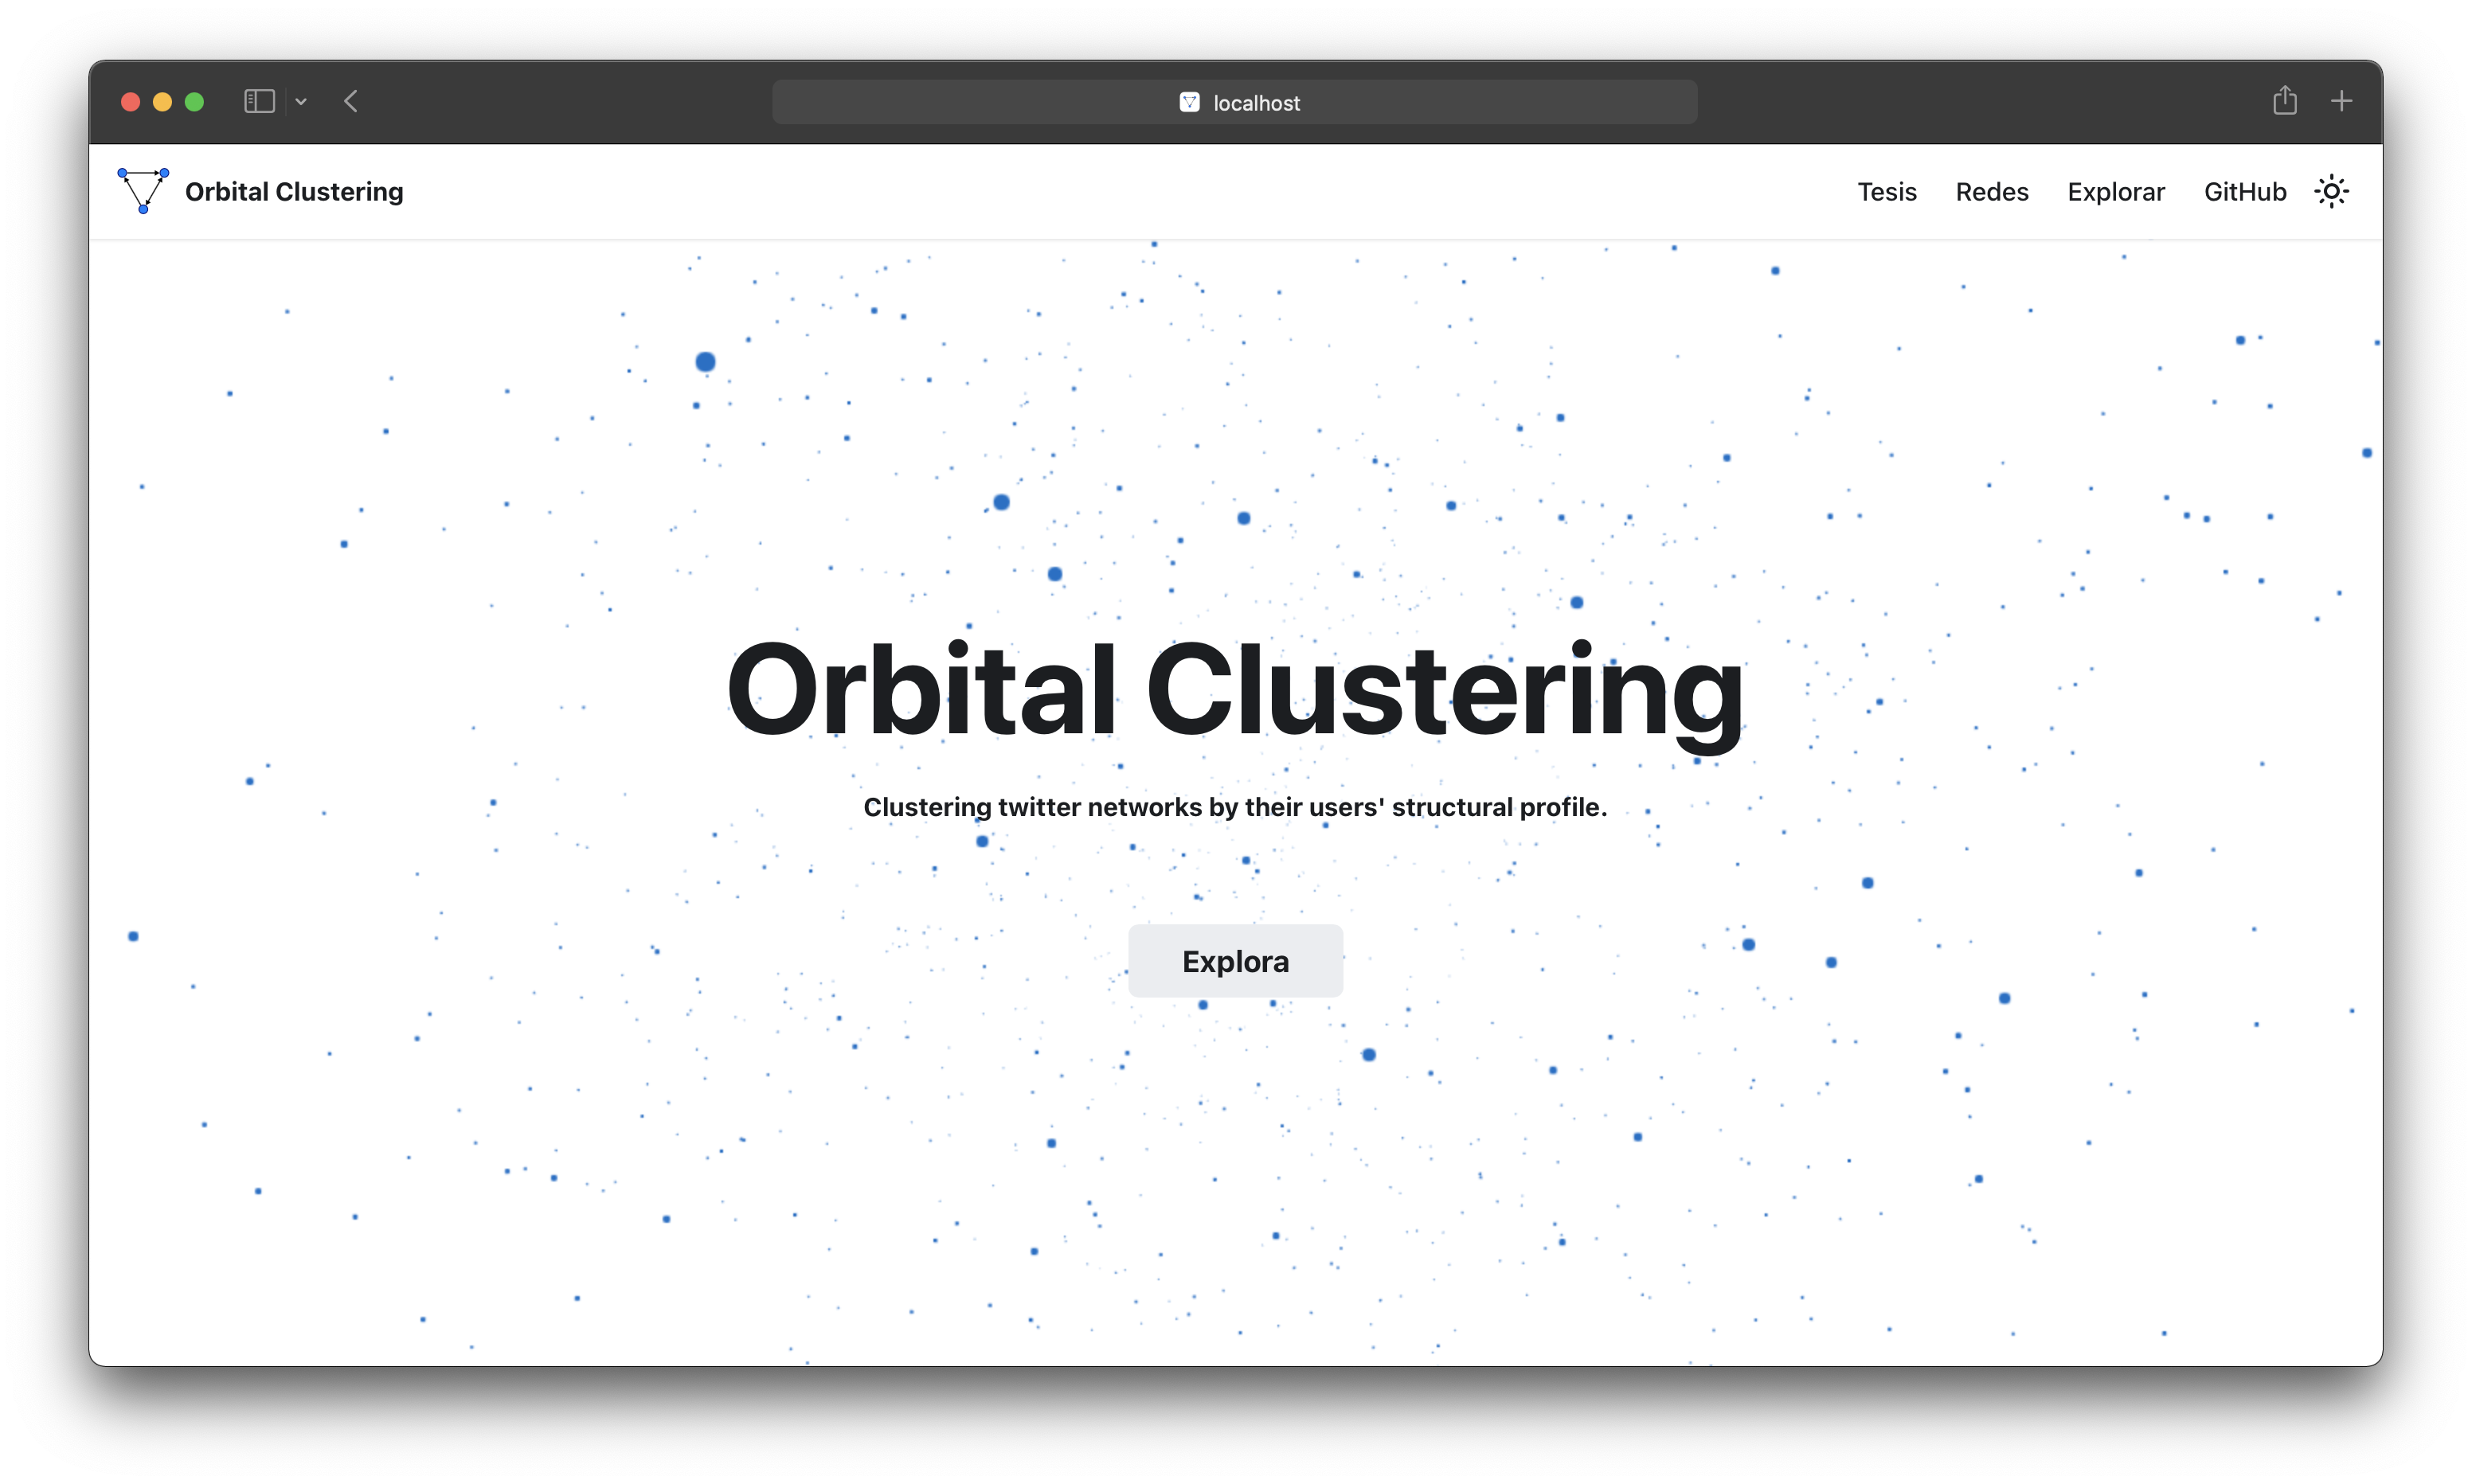
\includegraphics[width=1\textwidth]{images/web-main.png}
    \caption{Página principal de la herramienta web.}
    \label{img:web-main}
\end{figure}

La herramienta web tiene distintas pestañas que permiten explorar distintos aspectos del trabajo. La primera, permite explorar con una gráfica de radar la composición por tipo de usuarios de la red seleccionada. La \ref{img:web-comp} ejemplifica la composición de una red.

 \begin{figure}
   \centering
   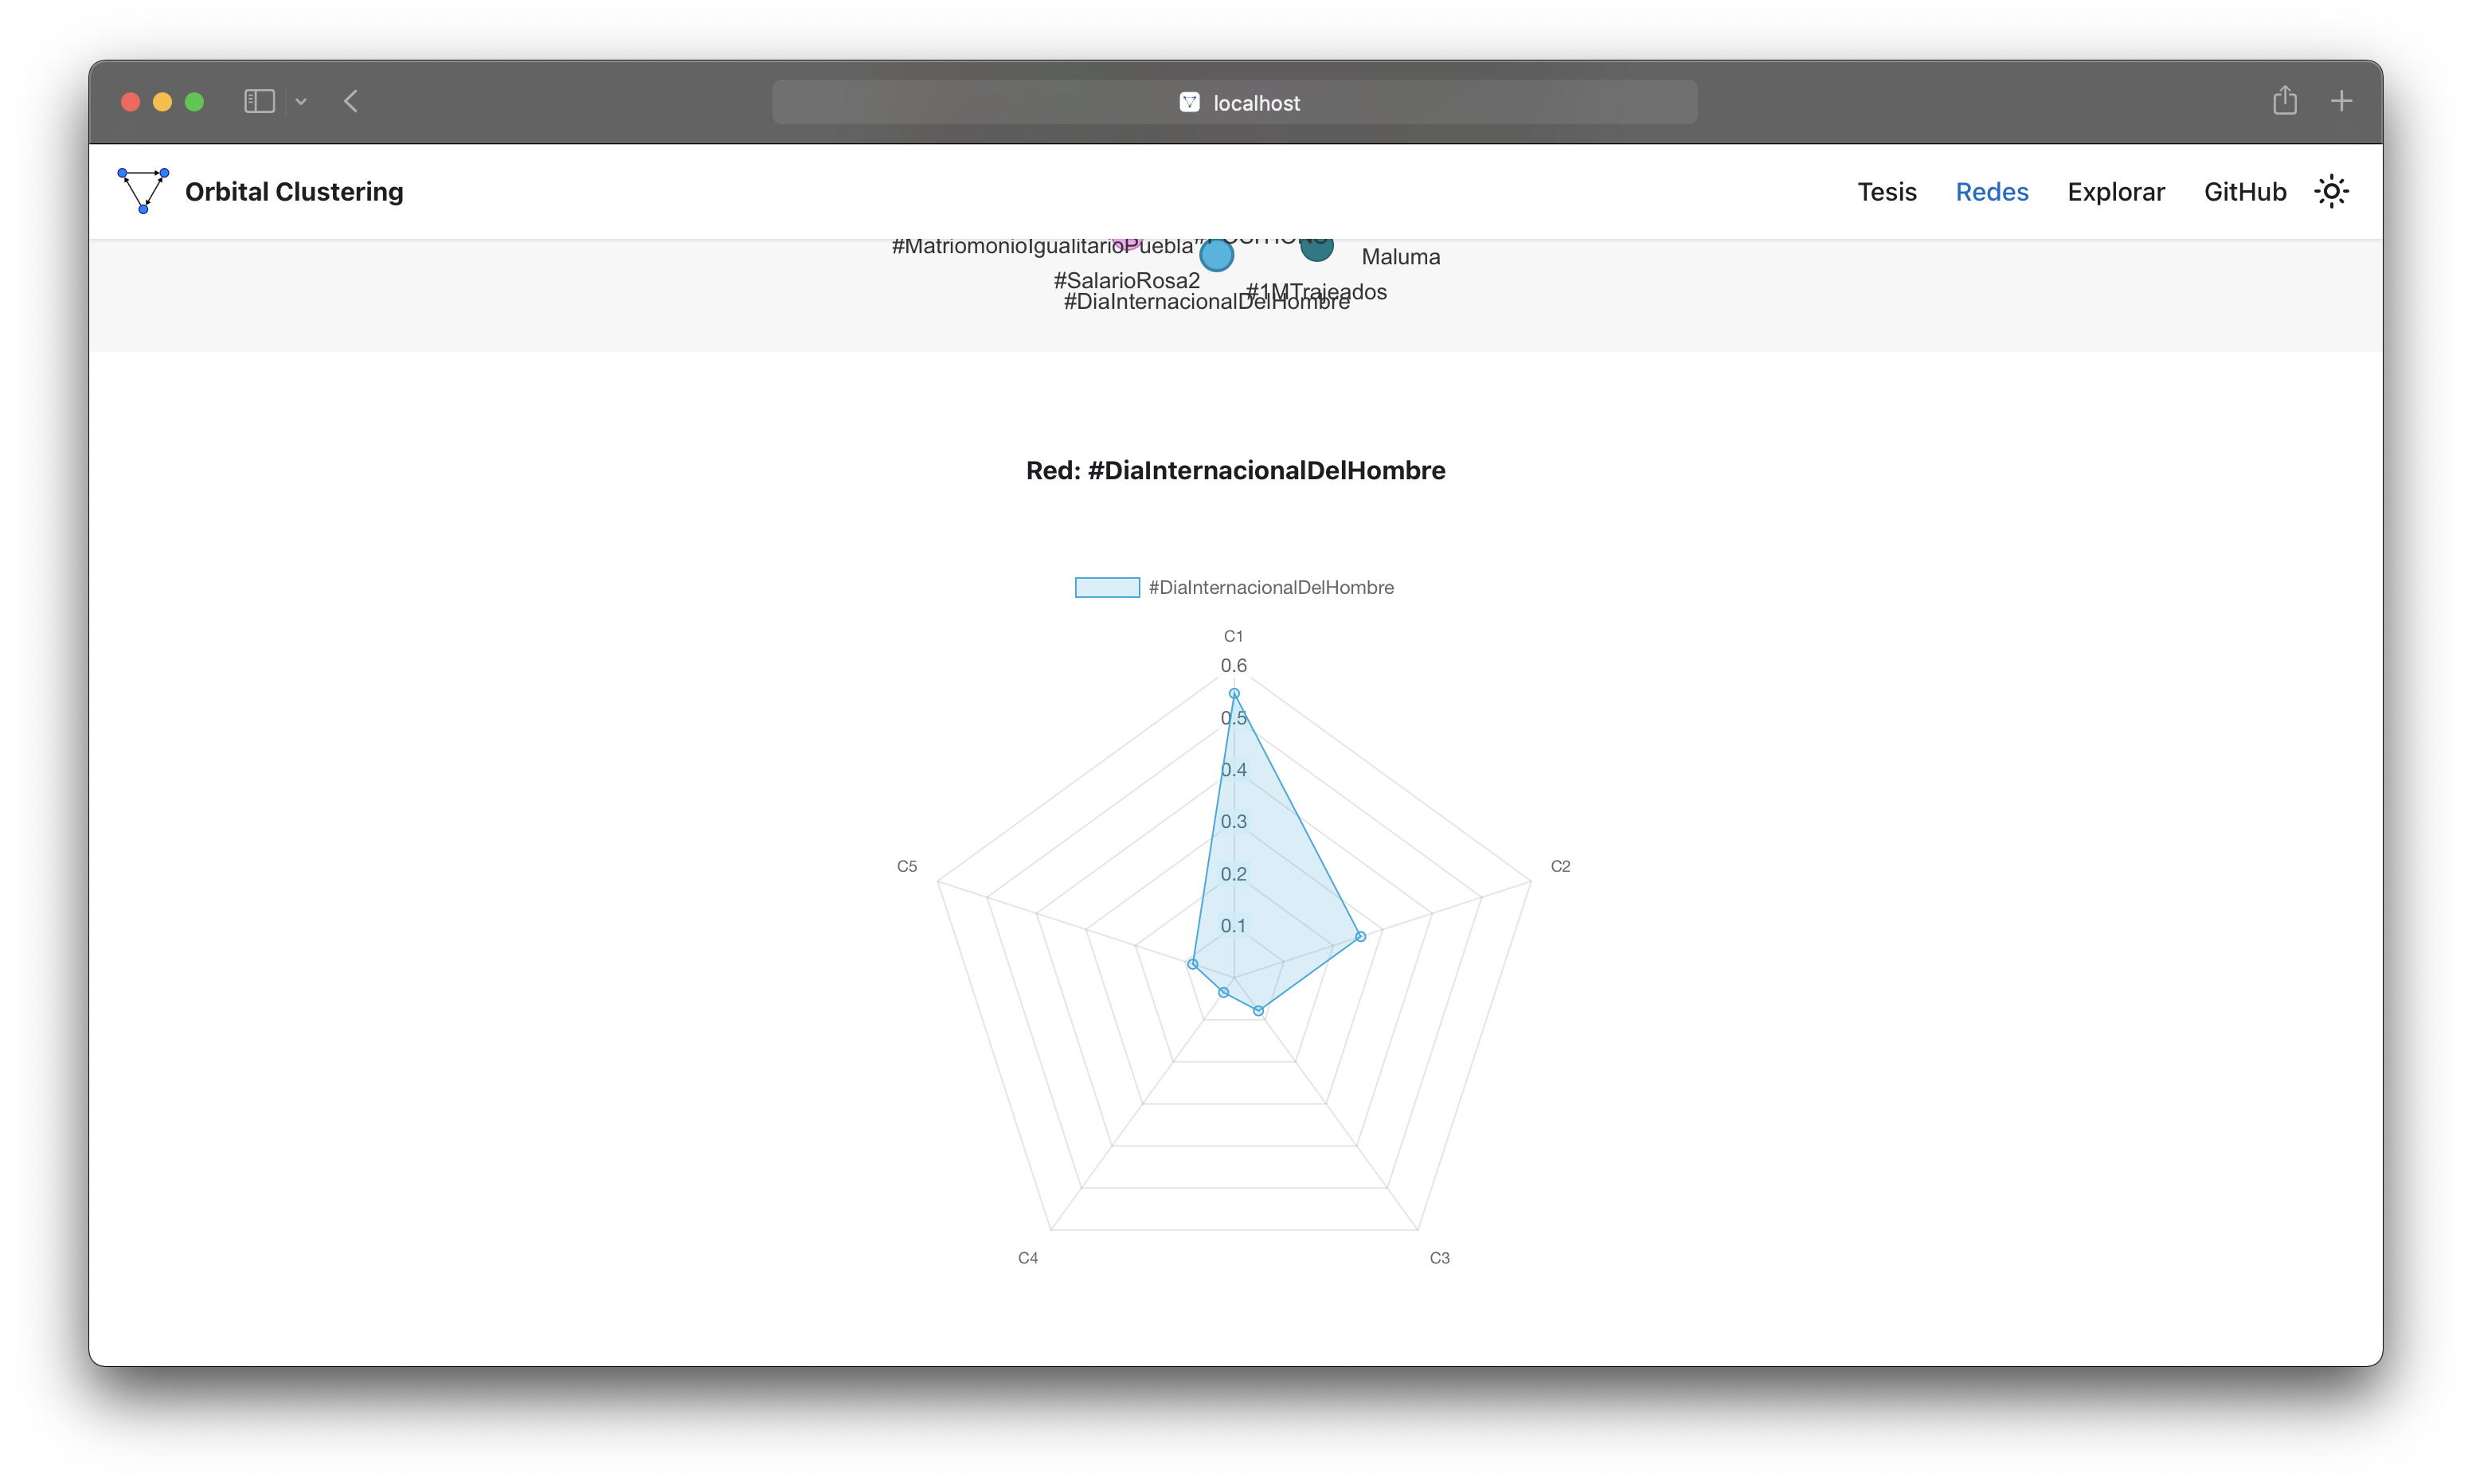
\includegraphics[width=1\textwidth]{images/web-comp.png}
    \caption{Ejemplo de la visualización de la composición de una red utilizando una gráfica de rada.}
    \label{img:web-comp}
\end{figure}

Otra de las funciones principales es la visualización de los grafos con sus respectivos nodos coloreados de acuerdo al perfil que pertenecen. La \ref{img:web-graph} nos muestra la red de Coco, esta visualización del grafo nos da algunas nociones sobre las interacciones dentro de la red.

 \begin{figure}
   \centering
   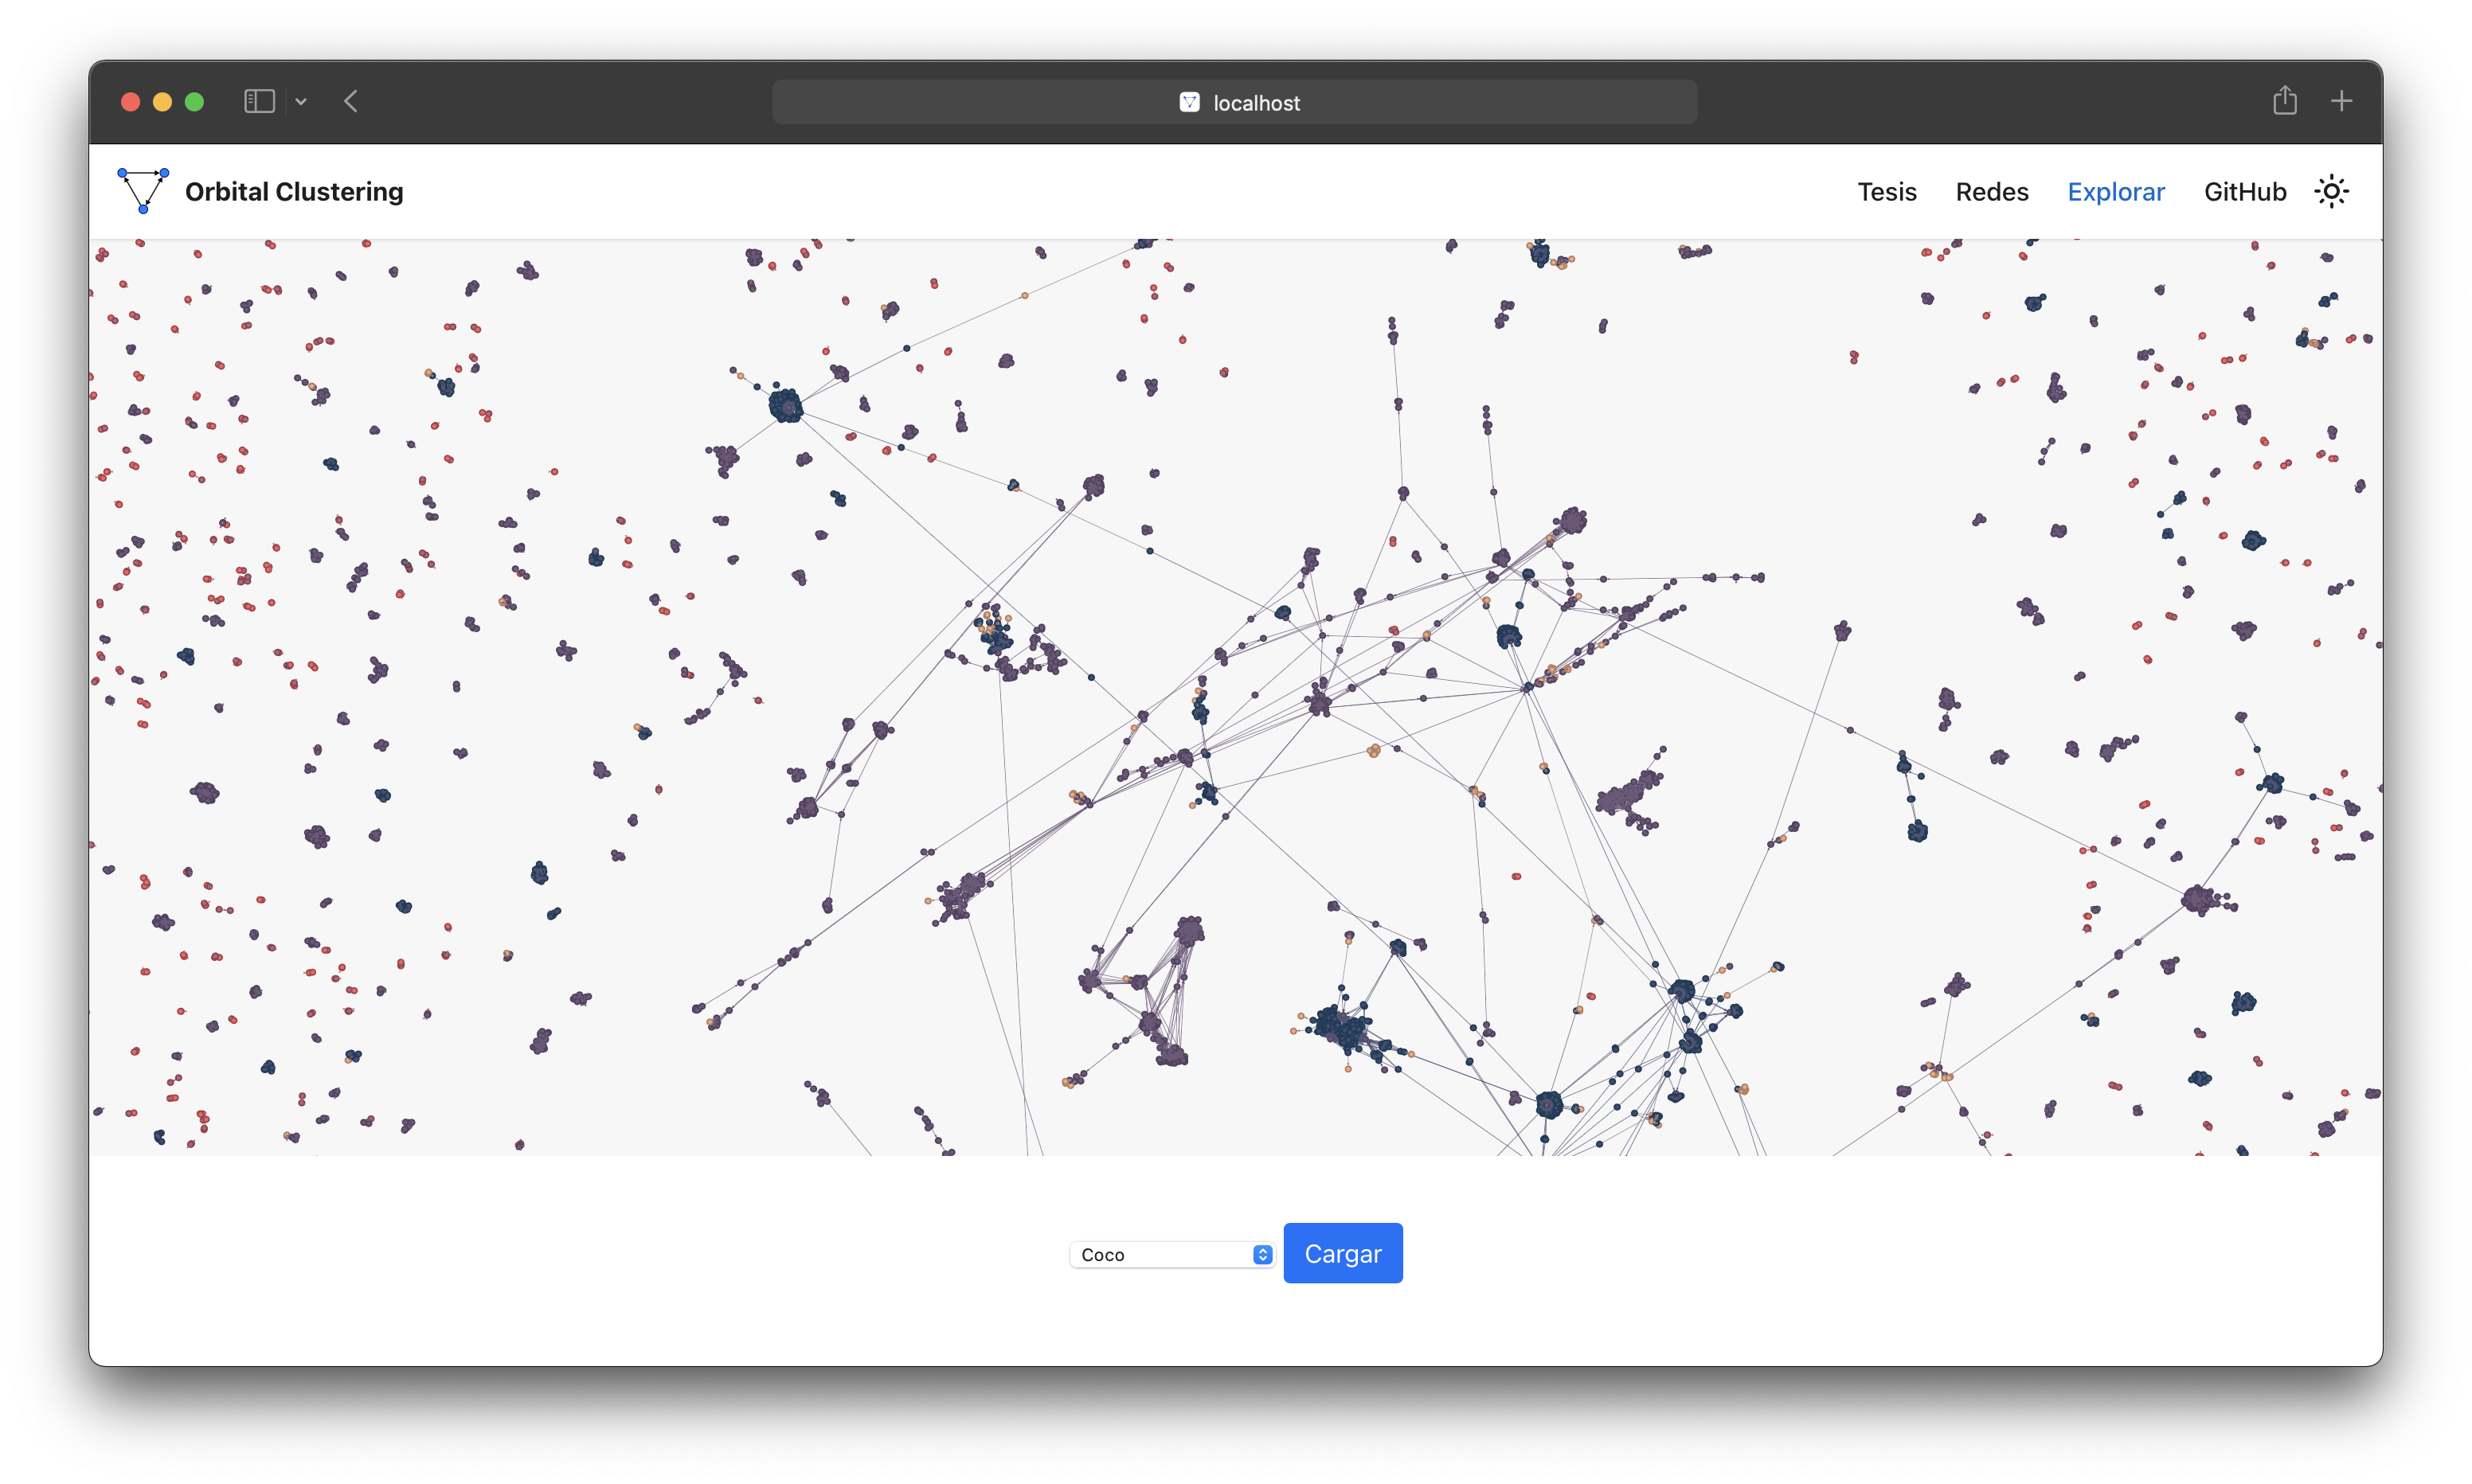
\includegraphics[width=1\textwidth]{images/web-graph.png}
    \caption{Ejemplo de la visualización de una red dentro de la herramienta web.}
    \label{img:web-graph}
\end{figure}

Los grafos que se presentan a continuación fueron escogidos al ser los más lejanos de acuerdo al agrupamiento jerárquico. En \ref{fig:net-salario} observamos la red correspondiente al \#Salario Rosa en las que la mayoría de las cuentas interactúan con un único usuario. Este tipo de comportamiento podría sugerir que el hashtag nace a partir de un gran influenciador o que se trata de cuentas automatizadas que tienen el objetivo de hacer central a un usuario en la red. En la \ref{fig:set-salario} podemos observar una red más bien fragmentada en la que no existe una conversación central.

\begin{figure}
    \centering
    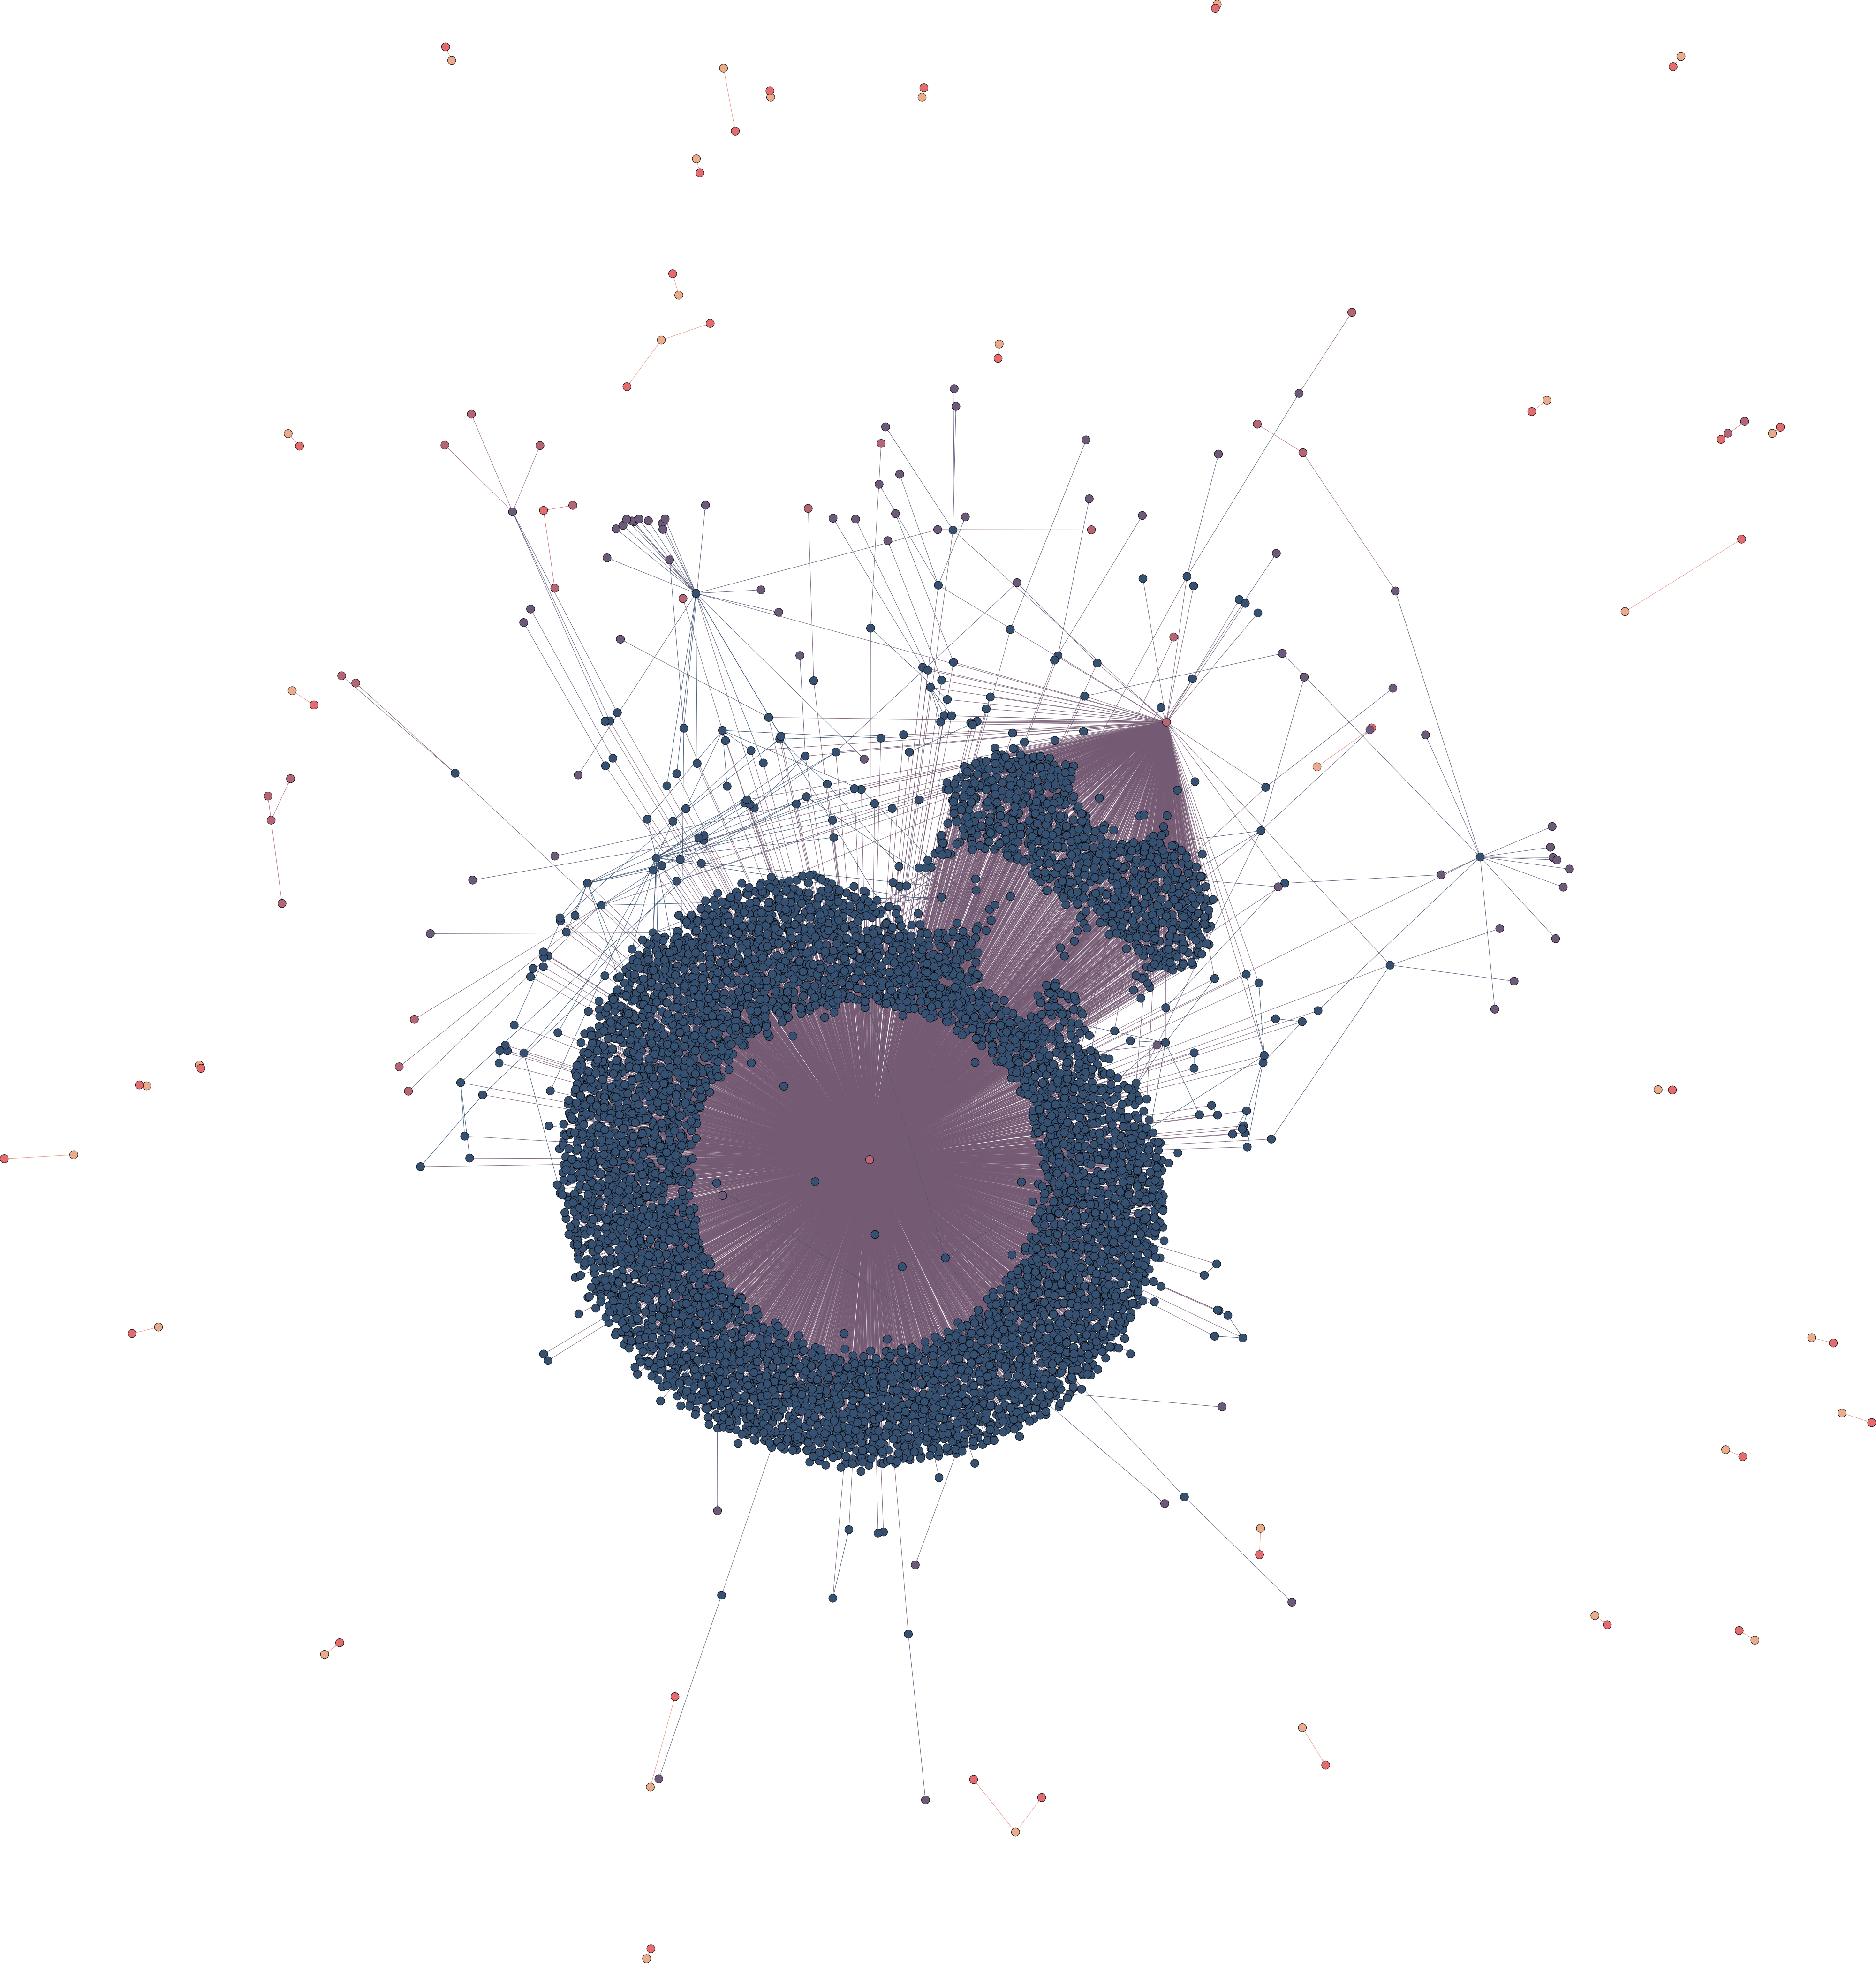
\includegraphics[width=.75\textwidth]{images/SalarioRosa.png}
    \caption{Red \#SalarioRosa2 coloreada respecto al grupo al que pertenece cada nodo en la red.}
    \label{fig:net-salario}
\end{figure}

\begin{figure}
    \centering
    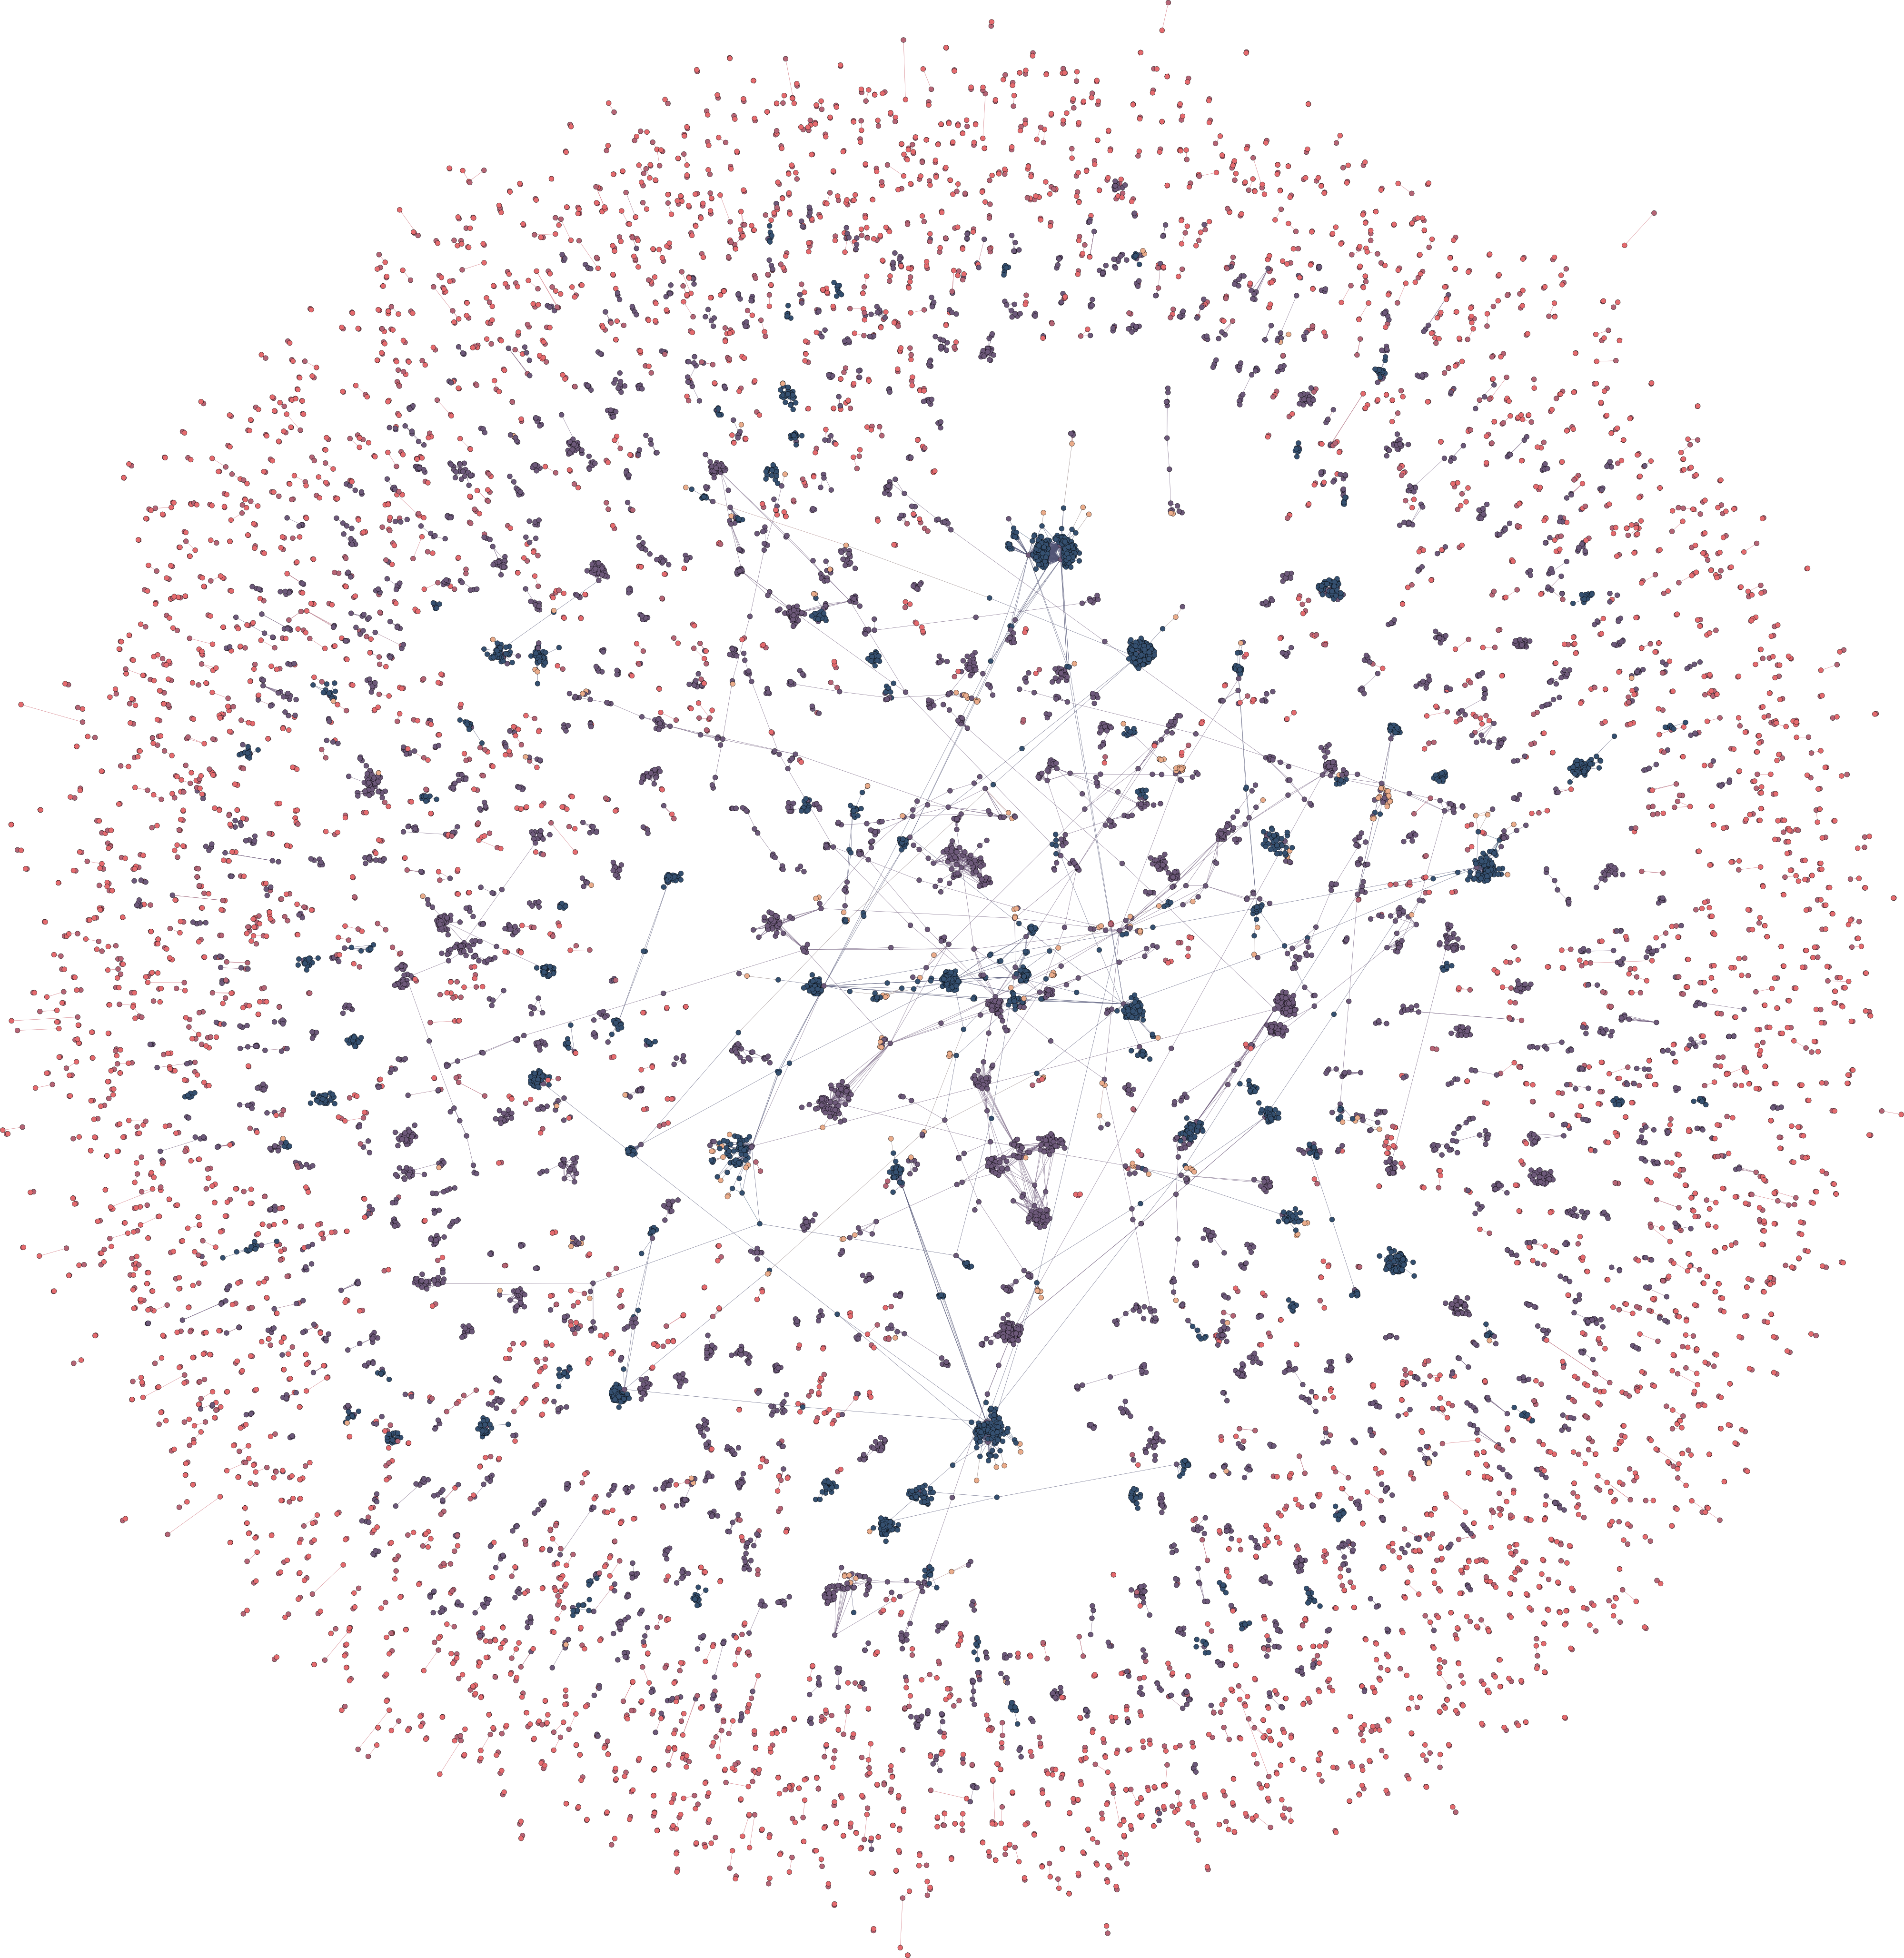
\includegraphics[width=.75\textwidth]{images/Coco.png}
    \caption{Red Coco coloreada respecto al grupo al que pertenece cada nodo en la red.}
    \label{fig:net-coco}
\end{figure}


\begin{table}[h]
    \begin{center}
        \csvautotabular{csv/embeddings-comp.csv}
        \caption{Comparación de los embeddings de las redes de Coco y \#SalarioRosa2}
    \end{center}
\end{table}


\section{Discusión}
En el conjunto de datos analizado, cuatro de los perfiles (1, 2, 4, 5) se distinguen por la presencia de una órbita dominante en el vector centroide representativo. En cambio, el grupo restante (3) tiene una distribución de órbitas más equilibrada en el vector de firmas de su centroide.

A continuación, se presenta una caracterización para cada uno de los perfiles de usuario identificados.  

\begin{itemize} 

\item \emph{Perfil 1, Esparcidor.} La órbita dominante es la 1, que desempeña el papel de un pozo en el graphlet compuesto por un solo arco. Las órbitas 2, 6 y 11 (todas ellas órbitas fuente) nunca aparecen en los vectores de firmas de estos usuarios. Analizando los vecindarios con tres nodos, las pocas veces que este perfil desempeña el papel de oyente, también lo hace de audiencia. Dada la alta frecuencia de la órbita dominante, es razonable suponer que estos usuarios producen información que motiva a los lectores a responder. \begin{figure}[htbp]
   \centering
   \includesvg[width=0.25\textwidth]{figures/G0.svg}
    \caption{Graphlet 0 y órbitas 0 y 1.}
    \label{img:web-comp}
\end{figure}

\item \emph{Perfil 2, Repetidor.} La órbita dominante es la 0, que desempeña el papel de oyente en un graphlet de arco, pero no tiene el papel de audiencia. La mayoría de las otras órbitas no aparecen asociadas a este tipo de usuario. En particular, si observamos todos los vecindarios con dos y tres nodos, este perfil nunca es retuiteado o mencionado por otro usuario. Además, observamos que el usuario no participa en graphlets de tamaño cuatro y, por tanto, tampoco en vecindarios más grandes. A partir de los roles recurrentes encontrados en esta órbita, podríamos decir que estos usuarios tienden a repetir los mensajes en la mayoría de sus interacciones sin impactar significativamente en la conversación. \begin{figure}[htbp]
   \centering
   \includesvg[width=0.25\textwidth]{figures/G0.svg}
    \caption{Graphlet 0 y órbitas 0 y 1.}
    \label{img:web-comp}
\end{figure}

\item \emph{Perfil 3, Conversador.} Las órbitas principales de este perfil incluyen las órbitas dominantes de las otras cuatro. Además, contiene las órbitas 7, 17, 21 y 31. Las tres primeras son oyentes, pero la órbita 31 desempeña todos los papeles de sumidero en un graphlet trinodo. La variedad de roles que puede adoptar este grupo de usuarios, se ve reflejada en la composición equilibrada de los vectores de firmas asociados, sugiere que este perfil permite el flujo de información hacia y desde los otros perfiles predominantes.
    
\item \emph{Perfil 4, Reportero.} La órbita dominante es la 29, que desempeña todos los papeles de oyente en el graphlet de un triodo. Esta órbita dominante desempeña el papel de oyente. Analizando los vecindarios con tres nodos, es infrecuente que este perfil participe en rutas con una longitud superior a uno o que responda a tweets de dos nodos diferentes, pero es habitual que el usuario responda a tweets que están siendo contestados por una o dos personas más. Así, podríamos decir que este tipo de usuario tiende a responder a tweets y usuarios que son populares. Dado que este perfil incluye todas las órbitas, podríamos decir que estos usuarios tienen más impacto en la conversación que los repetidores. \begin{figure}[htbp]
   \centering
   \includesvg[width=0.2\textwidth]{figures/G10.svg}
    \caption{Graphlet 10 y órbitas 29 y 30.}
    \label{img:web-comp}
\end{figure}

\item \emph{Perfil 5, Inconformista.} La órbita dominante es la 24, que desempeña el papel de hablante en un graphlet de 4 nodos. La particular arquitectura de este graphlet sugiere la presencia de nodos que recogen información de diferentes fuentes y que no interactúan entre sí. El comportamiento sugiere que este usuario participa en una discusión más amplia con un punto de vista parcial. \begin{figure}[htbp]
   \centering
   \includesvg[width=0.05\textwidth]{figures/G8.svg}
    \caption{Graphlet 8 y órbitas 21 a 24.}
    \label{img:web-comp}
\end{figure}

\end{itemize}

Las órbitas 30, 63, 85, 91, 105, 118 y 125 son hablantes con un grado de salida igual a 3, que aparecen con muy poca frecuencia en las firmas de los perfiles identificados. Es de esperar que estas órbitas aparezcan en usuarios reconocidos como \textit{Influencers} de la red. La presencia de la órbita 29 en el perfil de Reportero sugiere que la órbita 30 aparece varias veces en una red. Curiosamente, la órbita 30 aparece de forma distribuida, sin ser la órbita principal en los perfiles Locutor, Conversador o NonConformer.

En cuanto a la agrupación de las redes, la metodología propuesta puede ordenar la colección y definir grupos interpretables que proporcionan una visión de la dinámica originada por los diferentes temas. Los grupos no responden a una diferenciación temática, lo que refuerza la idea de que los procesos de difusión en Twitter no dependen sólo del contenido. No obstante, el análisis revela diferencias entre las redes con algunas que incluso muestran una clara variación en cuanto a la distribución del papel de los usuarios en la circulación de ideas a través de Twitter. 

En el grupo de las redes que muestran una alta inequidad en las opiniones propagadas (redes más a la izquierda en la Fig. \ref{fig:composition}), con unas pocas voces autorizadas (locutores) de las que se hacen eco otros perfiles (reporteros), encontramos algunas iniciativas gubernamentales (\#SalarioRosa, \#OfrendaEdoMex, \#TarjetaRosa). Podría darse el caso de que algunos tuits sean lanzados y manejados estratégicamente para aumentar su importancia. En el otro lado del espectro (instancias más a la derecha en la Fig. \ref{fig:composition}), encontramos redes temáticas relacionadas con películas y temas generales (Coco, Karol, FelizMiercoles) que abarcan un intercambio de información más distribuido, lo que sugiere un tema con un mayor nivel de participación y menos voces predominantes sobre el tema. 

